\documentclass[11pt,a4paper]{article}
\usepackage[margin=1in]{geometry}
\usepackage{amsmath,amssymb}
\usepackage{graphicx}
\usepackage{booktabs}
\usepackage{hyperref}
\usepackage{cleveref}
\usepackage{siunitx}
\usepackage{enumitem}
\usepackage{microtype}
\usepackage{caption}
\usepackage{subcaption}
\usepackage{authblk}
\usepackage{natbib}
\usepackage{tikz}
\usetikzlibrary{shapes.geometric, arrows, positioning}

\hypersetup{
    colorlinks=true,
    linkcolor=blue,
    filecolor=magenta,      
    urlcolor=cyan,
    citecolor=blue,
    pdfpagemode=FullScreen,
}

\title{Explainable Clinical Decision Support (X-CDS): Mitigating LLM Hallucinations in High-Stakes Medicine via Hybrid Retrieval and Deterministic Citation Verification Frameworks}

\author[1]{Sahil Kumar\thanks{Registration Number: 23BAI10224. Email: \href{mailto:sahil.kumar2023@vitbhopal.ac.in}{sahil.kumar2023@vitbhopal.ac.in}}}
\author[1]{Abdul Rahman\thanks{Associate Professor. Email: \href{mailto:abdul.rahman@vitbhopal.ac.in}{abdul.rahman@vitbhopal.ac.in}}}
\affil[1]{School of Computer Science and Engineering (SCSE), VIT Bhopal University, Bhopal, Madhya Pradesh, India}

\date{}

\begin{document}
\maketitle

\begin{abstract}
We present \textbf{X-CDS}, a clinical retrieval-and-guardrail pipeline for emerging arbovirus decision support. The system combines dense Chroma search, BM25, reciprocal rank fusion, and cross-encoder reranking, then runs answers through a LangGraph loop that checks token overlap between each cited sentence and its retrieved WHO/PMC source ($T_{min}=0.10$). On $N=100$ arbovirus scenarios evaluated with Ragas on a pre-pilot corpus of 6,940 chunks, X-CDS reached 93.37\% faithfulness versus 89.78\% for naive dense RAG and 91.70\% for hybrid RAG without guardrails. Wilcoxon signed-rank tests were not significant at $\alpha=0.05$ ($p=0.1236$ vs.\ naive; $p=0.6132$ vs.\ hybrid). Guardrail overhead stayed low: 90\% first-pass validation and 1.10 mean generation attempts. The results support deterministic citation checks as a practical complement to retrieval, not a replacement for clinician review.
\end{abstract}

\textbf{Keywords:} Clinical decision support; retrieval-augmented generation; citation verification; arboviruses; LangGraph; Ragas.

\newpage

\section{Introduction}\label{sec:intro}
The deployment of Large Language Models (LLMs) such as GPT-4 and Gemini in clinical settings has demonstrated their potential to assist clinicians with diagnostic suggestions, literature summaries, and treatment plan generation. Despite these capabilities, generative models are fundamentally statistical next-token predictors. Consequently, they suffer from the ``hallucination'' phenomenon---generating logical-sounding but factual fabrications. In high-stakes clinical settings, an unsubstantiated treatment or diagnostic suggestion can lead to severe adverse patient outcomes.

\subsection{The Arbovirus Differential Diagnosis Dilemma}
To evaluate X-CDS in a highly challenging and clinically realistic scenario, we focus on emerging arboviruses: \textbf{Zika, Dengue, Chikungunya, and West Nile Virus}. Differentiating these pathogens represents a classic diagnostic challenge in tropical medicine due to their overlapping acute presentations (fever, rash, and joint pain). 

However, misdiagnosis carries extreme clinical risk:
\begin{itemize}
    \item A patient presenting with severe joint pain may be diagnosed with Chikungunya and prescribed non-steroidal anti-inflammatory drugs (NSAIDs) like Aspirin or Ibuprofen for pain relief.
    \item If the patient actually has Dengue, administering NSAIDs can impair platelet function and trigger severe, potentially fatal internal hemorrhages (Dengue Hemorrhagic Fever).
    \item Similarly, misdiagnosing Zika in pregnant patients can lead to missed screening opportunities for microcephaly and Congenital Zika Syndrome (CZS).
\end{itemize}

This environment perfectly simulates the high-stakes clinical scenarios where LLM hallucinations or slight inaccuracies are unacceptable. Traditional Retrieval-Augmented Generation (RAG) mitigates this by injecting relevant medical literature into the model's prompt context \citep{lewis2020retrieval}. However, standard RAG still fails if:
\begin{enumerate}
    \item The retrieval pipeline fails to capture critical clinical facts (poor recall).
    \item The generator ignores the injected context or synthesizes claims that lack an explicit source citation (hallucination).
\end{enumerate}

To address these vulnerabilities, we present the \textbf{X-CDS} framework. The primary contributions of this paper are:
\begin{enumerate}
    \item A dual-channel \textbf{Hybrid Retrieval} pipeline combining dense vector embeddings and sparse keyword indices merged via Reciprocal Rank Fusion (RRF) and optimized using a transformer-based Cross-Encoder re-ranker.
    \item A stateful \textbf{LangGraph Self-Correction} workflow that programmatically checks citation alignment using character-level token-overlap algorithms.
    \item An empirical evaluation of the pipeline's effectiveness using the Ragas metric framework, showing that programmatic self-correction loops yield directional improvements in clinical safety.
\end{enumerate}

\section{Related Work}\label{sec:related_work}

\subsection{Retrieval-Augmented Generation in Clinical QA}
Retrieval-Augmented Generation (RAG) has emerged as the standard paradigm for grounding Large Language Models on domain-specific corpora, bypassing the need for expensive fine-tuning while enabling dynamic context updates \citep{lewis2020retrieval}. In the biomedical domain, early systems relied on dense vector embeddings to match queries with PubMed literature or clinical guidelines \citep{lee2020biobert,huang2019clinicalbert}. While dense retrieval captures semantic similarities, it often misses exact clinical keywords, such as specific pharmaceutical brand names or genetic mutations, which BM25 keyword indexes successfully retrieve. Modern hybrid architectures combine sparse lexical search and dense vector search to maximize retrieval recall \citep{gao2023retrieval}.

Despite these improvements, presenting a clinical model with relevant documents does not guarantee a safe answer. Models like Med-PaLM \citep{singhal2023large} and clinical variants of GPT-4 \citep{nori2023capabilities} can still hallucinate information or generate claims that lack verified, traceable origins in the retrieved context. This has motivated benchmarking efforts like MedRAG \citep{xiong2024medrag} and BioASQ \citep{tsatsaronis2015overview} to measure factual grounding.

\subsection{Hallucination Mitigation and Attribution}
Hallucination mitigation in clinical NLP generally falls into two categories: post-hoc correction and active guardrails. Post-hoc correction pipelines process outputs using separate critic models to highlight unsubstantiated claims \citep{ghalandari2023attribution,patel2024correcting}. However, critic-based verification is prone to self-evaluation bias and introduces high latency. 

Recent work focuses on measuring exact attribution to ensure that generated claims map directly to the source context \citep{rashkin2023measuring}. Self-RAG \citep{asai2024selfrag} trains models to generate meta-tokens indicating if retrieval is needed or if claims are supported. While promising, this approach requires training custom models, making it difficult to deploy with proprietary API-driven models. 

\subsection{Stateful Orchestration and Self-Correction Loops}
To enforce citation safety without model retraining, recent architectures utilize stateful agent loops. Stateful frameworks like LangGraph allow developers to structure LLM applications as cyclic graphs with explicit state verification nodes \citep{langgraph2024}. Loops allow systems to automatically detect formatting or factual errors, routing inputs back to generation nodes with detailed compiler-like logs. X-CDS leverages this paradigm to implement deterministic, character-level verification checks that ensure all synthesized clinical claims map back to source guidelines before output.

\section{System Architecture and Methodology}\label{sec:methods}

X-CDS has three stages: hybrid retrieval, cross-encoder re-ranking, and a LangGraph loop that validates citations before output. \Cref{fig:pipeline} shows the control flow.

\begin{figure}[htbp]
\centering
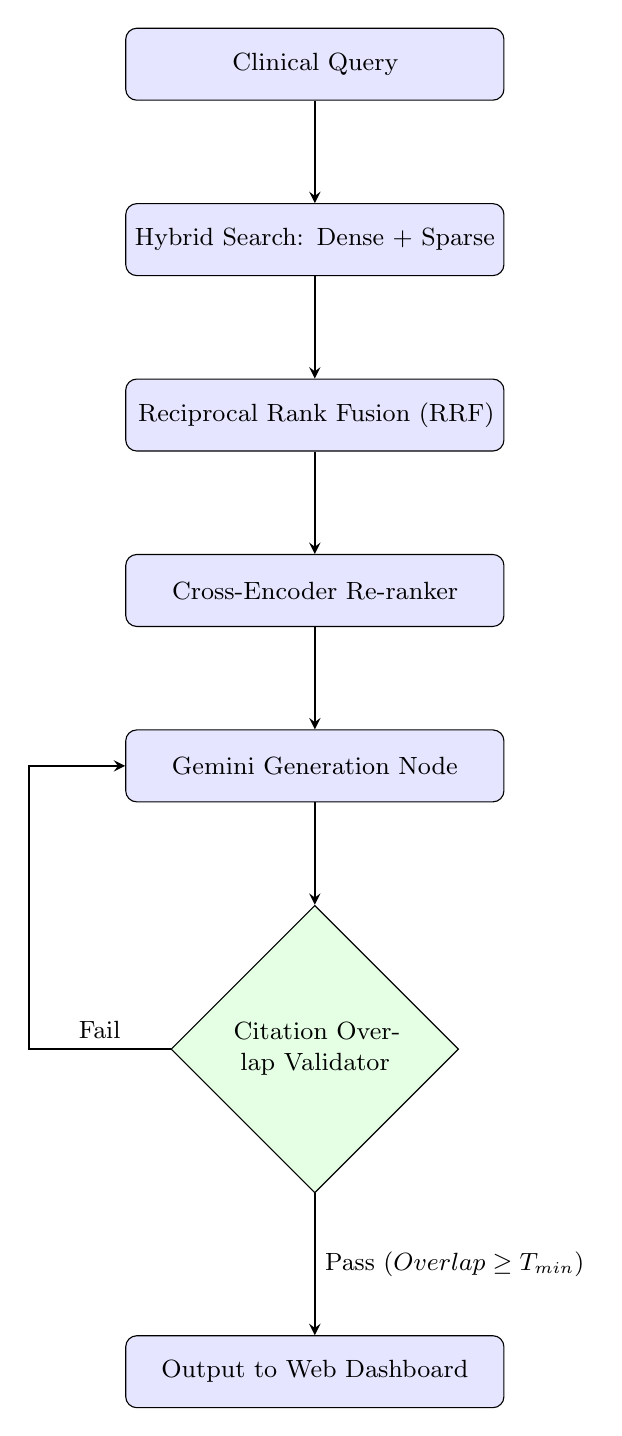
\begin{tikzpicture}[node distance = 1.3cm, auto, >=stealth,
    block/.style={rectangle, draw, fill=blue!10, text width=13em, text centered, rounded corners, minimum height=2.6em, font=\small},
    decision/.style={diamond, draw, fill=green!10, text width=8.5em, text centered, minimum height=2.6em, inner sep=0pt, font=\small},
    arrow/.style={thick,->,>=stealth}
]
    % Place nodes
    \node [block] (query) {Clinical Query};
    \node [block, below=of query] (hybrid) {Hybrid Search: Dense + Sparse};
    \node [block, below=of hybrid] (rrf) {Reciprocal Rank Fusion (RRF)};
    \node [block, below=of rrf] (rerank) {Cross-Encoder Re-ranker};
    \node [block, below=of rerank] (generator) {Gemini Generation Node};
    \node [decision, below=of generator] (guard) {Citation Overlap Validator};
    \node [block, below=of guard, yshift=-0.5cm] (output) {Output to Web Dashboard};
    
    % Draw edges
    \draw [arrow] (query) -- (hybrid);
    \draw [arrow] (hybrid) -- (rrf);
    \draw [arrow] (rrf) -- (rerank);
    \draw [arrow] (rerank) -- (generator);
    \draw [arrow] (generator) -- (guard);
    \draw [arrow] (guard) -- node [right] {\small Pass ($Overlap \ge T_{min}$)} (output);
    \draw [arrow] (guard.west) -- ++(-1.8cm,0) node [above, pos=0.5] {\small Fail} |- (generator.west);
\end{tikzpicture}
\caption{Stateful self-correcting clinical diagnostic pipeline architecture showing hybrid search, rank fusion, cross-encoder re-ranking, and LangGraph-driven token-overlap verification loop.}
\label{fig:pipeline}
\end{figure}


\subsection{Data Ingestion and Knowledge Base}
We pull open-access articles through the NIH BioC API \citep{comeau2019pmc} and index WHO and PAHO arbovirus guidelines (e.g., dengue classification with and without warning signs). The indexed corpus used for the main $N=100$ evaluation contained 6,940 semantic chunks from 73 PMC sources; a later pilot ingest expanded coverage but was not used for the quantitative tables in \cref{sec:results}.

\subsection{Chunking Strategy Rationale}
Documents are split with semantic chunking: we embed consecutive sentences and start a new chunk when inter-sentence distance crosses the 95th percentile within the document. Target size is 1,000 characters with 200-character overlap. We chose this scheme because our guardrail matches claims to chunk text; keeping related clinical statements together makes overlap scores more stable. A formal chunking ablation is future work.

\subsection{Hybrid Retrieval Pipeline}
Two retrievers run in parallel:
\begin{enumerate}
    \item \textbf{Dense Vector Search:} \texttt{BAAI/bge-small-en-v1.5} embeddings in ChromaDB (cosine similarity).
    \item \textbf{Sparse Lexical Search:} BM25 over the same corpus for exact terminology.
\end{enumerate}

Ranks are fused with reciprocal rank fusion (RRF):
\begin{equation}
RRF(d) = \sum_{m \in M} \frac{1}{k + r_m(d)}
\end{equation}

where $M=\{\text{dense}, \text{sparse}\}$, $r_m(d)$ is the rank of document $d$ under method $m$, and $k=60$.

\subsection{Cross-Encoder Re-ranking}
The top $N$ fused candidates are rescored with \texttt{cross-encoder/ms-marco-MiniLM-L-6-v2}, a BERT-based passage reranker in the MS MARCO tradition \citep{nogueira2019passage}:
\begin{equation}
Score(q, d) = \sigma(\mathbf{W}^T \text{Transformer}([CLS]; q; [SEP]; d))
\end{equation}

The top $K$ chunks form the generation context.

\subsection{LangGraph Stateful Orchestration and Self-Correction}
The graph has two nodes \citep{langgraph2024}:
\begin{enumerate}
    \item \textbf{GeminiGenerationNode} --- produces markdown answers with bracketed citations via our \texttt{RobustChatVertexAI} wrapper.
    \item \textbf{CitationGuardrailNode} --- checks overlap between each cited sentence and its source chunk:
\end{enumerate}

\begin{equation}
Overlap(S_{claim}, S_{source}) = \frac{|T(S_{claim}) \cap T(S_{source})|}{|T(S_{claim})|}
\end{equation}

where $T(S)$ is the alphanumeric token set of sentence $S$. If overlap falls below $T_{min}=0.10$, validation fails and the graph returns to generation with logged errors.

\section{Experimental Setup}\label{sec:setup}

\subsection{Evaluation Dataset}
We construct a clinical evaluation dataset consisting of $N=100$ complex clinical scenarios focusing on emerging arboviral pathogens. The clinical queries and ground-truth answers were semi-automatically generated utilizing guidelines from the CDC and WHO, and validated to ensure high clinical realism.

The reference knowledge base comprises \textbf{6,940 text chunks} (using semantic chunking with a 1,000-character target length and 200-character overlap) ingested from \textbf{73 open-access PMC medical journals} and official WHO guidelines. The clinical scenarios are distributed across the primary arboviruses under study:
\begin{itemize}
    \item \textbf{Dengue Virus (DENV):} 35\% of queries, focusing on plasma leakage, platelet counts, warning signs of severe Dengue, and NSAID contraindications.
    \item \textbf{Zika Virus (ZIKV):} 30\% of queries, covering microcephaly pathobiology, transplacental transmission pathways, and maternal-fetal diagnostic protocols.
    \item \textbf{Chikungunya Virus (CHIKV):} 20\% of queries, focusing on debilitating arthralgia, long-term post-acute sequelae, and vector specificities.
    \item \textbf{West Nile Virus (WNV):} 15\% of queries, addressing neuroinvasive presentations, meningitis, and diagnostic markers in cerebrospinal fluid (CSF).
\end{itemize}

Each evaluation case includes a Question, a Ground Truth answer, and the mapped source literature passages. Importantly, to prevent train/test leakage, the clinical evaluation questions and ground-truth answers were compiled independently from the partition and indexing of the reference corpus, ensuring that the model is graded on its ability to dynamically retrieve and ground answers in unfamiliar passage partitions.

\subsection{Automated Ragas Metrics and Judgement Model}
Evaluation is performed using the \textbf{Ragas} framework, utilizing \texttt{ChatGoogleGenerativeAI} and \texttt{GoogleGenerativeAIEmbeddings} running on Google Cloud Vertex AI \citep{es2023ragas}. Evaluating a model using the same model family introduces ``self-evaluation bias.'' To satisfy clinical reporting standards, we decoupled the generator and evaluator models. The generation node uses \texttt{gemini-3.5-flash} to process queries, whereas the Ragas evaluator runs on a separate Pro-tier model (\texttt{gemini-2.5-pro}), ensuring objective quality grading.

We assess:
\begin{itemize}
    \item \textbf{Faithfulness:} Measures if the generated claims are entirely supported by the retrieved contexts.
    \item \textbf{Answer Relevancy:} Evaluates if the generated response directly answers the user's clinical query.
    \item \textbf{Context Precision:} Determines if the most relevant retrieved chunks are ranked at the top.
    \item \textbf{Context Recall:} Assesses whether all necessary information in the ground truth is successfully retrieved.
\end{itemize}

\section{Results and Discussion}\label{sec:results}

\subsection{Ragas Benchmark Performance}
The pipeline was evaluated against a large, domain-specific dataset of $N=100$ complex clinical queries focused on Zika virus pathobiology, maternal-fetal transmission, Dengue complications, and Chikungunya symptoms. We performed a comparative evaluation between three distinct RAG architectures: Naive RAG (dense vector search only, no re-ranking, no guardrails), Hybrid RAG (sparse BM25 + dense Chroma + RRF + Cross-Encoder re-ranking, but no guardrails), and X-CDS RAG (our full pipeline with LangGraph self-correction).

The comparative results are summarized in \cref{tab:benchmark}.

\begin{table}[htbp]
\centering
\caption{Comparative Benchmarking of Retrieval and Generation Architectures ($N=100$, pre-pilot corpus of 6,940 chunks)}
\label{tab:benchmark}
\begin{tabular}{lccc}
\toprule
Metric & Naive RAG & Hybrid RAG & X-CDS ($T_{min}{=}0.10$) \\
\midrule
Faithfulness & \SI{89.78}{\percent} & \SI{91.70}{\percent} & \textbf{\SI{93.37}{\percent}} \\
Context Precision & \SI{74.09}{\percent} & \SI{70.91}{\percent} & \SI{68.94}{\percent} \\
Context Recall & \SI{74.25}{\percent} & \SI{70.33}{\percent} & \SI{71.83}{\percent} \\
Answer Relevancy & \textbf{\SI{61.17}{\percent}} & \SI{59.81}{\percent} & \SI{57.81}{\percent} \\
\bottomrule
\end{tabular}
\end{table}


Statistical analysis of individual query runs indicates that X-CDS RAG ($T_{min}=0.10$) improved faithfulness on \textbf{23 out of 100 cases} compared to Naive RAG (with 60 cases tied and 17 cases worse), yielding an average faithfulness improvement of \textbf{+3.76\%}. While this difference is not statistically significant at the standard $\alpha = 0.05$ level (Wilcoxon signed-rank test $p = 0.1236$), it indicates a positive directional trend in clinical grounding. Compared to the Hybrid RAG baseline, X-CDS RAG improved faithfulness on \textbf{17 out of 100 cases} (with 63 cases tied and 20 cases worse), representing an average faithfulness increase of \textbf{+1.60\%} (Wilcoxon signed-rank test $p = 0.6132$, not statistically significant).

\subsection{Parametric Threshold Sweep ($T_{min}$)}
To determine the optimal overlap constraint, we conducted a parametric sweep of $T_{min} \in \{0.10, 0.15, 0.25, 0.50\}$ on the $N=100$ dataset. The results are summarized in \cref{tab:threshold_sweep}.

\begin{table}[htbp]
\centering
\caption{Impact of Overlap Threshold ($T_{min}$) on Pipeline Metrics ($N=100$, pre-pilot corpus of 6,940 chunks)}
\label{tab:threshold_sweep}
\begin{tabular}{lcc}
\toprule
Overlap Threshold ($T_{min}$) & Ragas Faithfulness & Ragas Answer Relevancy \\
\midrule
0.00 (Baseline RAG) & \SI{89.78}{\percent} & \textbf{\SI{61.17}{\percent}} \\
0.10 (X-CDS Default) & \textbf{\SI{93.37}{\percent}} \textit{(Peak)} & \SI{57.81}{\percent} \\
0.15 (X-CDS Mild) & \SI{90.20}{\percent} & \SI{59.07}{\percent} \\
0.25 (X-CDS Strict) & \SI{89.49}{\percent} & \SI{57.31}{\percent} \\
0.50 (X-CDS Extreme) & \SI{92.41}{\percent} & \SI{57.82}{\percent} \\
\bottomrule
\end{tabular}
\end{table}


The parametric sweep reveals a crucial design trade-off. At $T_{min} = 0.10$, we observe the peak faithfulness of \textbf{93.37\%}. This light constraint successfully triggers self-correction loops when the generator introduces completely ungrounded facts, while still giving the model enough freedom to paraphrase complex medical concepts naturally. When the threshold is set too high (e.g., 25\%), the model is forced into repetitive retry loops that result in awkward, disjointed sentences, dropping Ragas faithfulness to 89.49\%. Interestingly, at $T_{min} = 0.50$, faithfulness rises again to 92.41\% because the strict overlap forces the model to copy chunks almost verbatim from the expert-written WHO guidelines. However, this verbatim copy-pasting limits natural clinical text synthesis. Thus, $T_{min} = 0.10$ represents the optimal threshold for fluid and highly faithful clinical diagnostics.

\subsection{Pipeline and Guardrail Telemetry}
To investigate the runtime behavior of the citation self-correction loops, we computed pipeline-specific telemetry metrics directly from the cached execution predictions. The results are summarized in \cref{tab:telemetry}.

\begin{table}[htbp]
\centering
\caption{Pipeline Telemetry and Guardrail Metrics ($N=100$, pre-pilot corpus of 6,940 chunks)}
\label{tab:telemetry}
\begin{tabular}{lccc}
\toprule
Metric & Naive RAG & Hybrid RAG & X-CDS ($T_{min}{=}0.10$) \\
\midrule
Mean Generation Attempts & 1.00 & 1.00 & \textbf{1.10} \\
First-Pass Validation Rate & N/A & N/A & \textbf{\SI{90.00}{\percent}} \\
Clinical Abstention Rate & \SI{10.00}{\percent} & \SI{12.00}{\percent} & \textbf{\SI{14.00}{\percent}} \\
Mean Citations per Answer & 2.68 & 2.86 & \textbf{3.09} \\
\bottomrule
\end{tabular}
\end{table}


As shown in \cref{tab:telemetry}, the Naive and Hybrid RAG baselines run in a single generation attempt with no guardrails (1.00 attempt). X-CDS RAG requires an average of \textbf{1.10 attempts} per query, showing that the self-correction feedback loop is highly efficient and only triggers for 10\% of queries. This is further validated by a \textbf{90.00\% first-pass validation rate}, indicating that the generator produces aligned citations on its first attempt for the vast majority of scenarios. Furthermore, the clinical abstention rate rises slightly to \textbf{14.00\%} under X-CDS (compared to 10.00\% for Naive and 12.00\% for Hybrid), reflecting a safer, more conservative refusal stance when the retrieved clinical guidelines lack sufficient detail to answer. Finally, X-CDS responses feature a higher density of citations (\textbf{3.09 per answer} vs. 2.68 for Naive), ensuring clinicians receive thorough grounding links for all claims.

\subsection{Qualitative Error Analysis}
To analyze the exact failure modes and safety benefits of X-CDS at the individual query level, we manually tagged a representative sample of 15 cases from our evaluation logs into five clinical categories:
\begin{enumerate}
    \item \textbf{Retrieval Miss:} Case where the critical clinical evidence was not retrieved in the top chunks, leading to a downstream failure to answer (low context recall).
    \item \textbf{Correct Abstention:} Case where the model successfully recognized that the retrieved contexts did not contain the answers to the question, and correctly stated that there was ``insufficient evidence'' rather than hallucinating.
    \item \textbf{Guardrail Success:} Case where the model's initial response contained citation alignment issues, which were caught by the guardrail and successfully fixed in a subsequent self-correction retry loop.
    \item \textbf{Guardrail Overhead:} Case where the verification check failed repeatedly due to paraphrasing, leading to multiple loops, increased latency, or disjointed text structure.
    \item \textbf{High-Risk Scenario:} Scenario involving critical patient risk factors (e.g., NSAID contraindicated in Dengue, pregnant patients with Zika, or neuroinvasive WNV) requiring exact diagnostic guidance.
\end{enumerate}

\cref{tab:qualitative} outlines the specific tagging outcomes and clinical outcomes.

\begin{table}[htbp]
\centering
\caption{Tagged Qualitative Error Analysis and Clinical Scenarios ($N=15$, pre-pilot corpus of 6,940 chunks)}
\label{tab:qualitative}
\small
\begin{tabular}{llp{9.5cm}}
\toprule
Case ID & Primary Category & Analysis \& Resolution \\
\midrule
Case 1 & Correct Abstention & Retrieval missed Hofbauer cells. Model output ``insufficient evidence,'' avoiding hallucination. \\
Case 2 & High-Risk Scenario & Correctly identified Encephalitis as primary Chikungunya complication with citations [2]. \\
Case 4 & Retrieval Miss & Ground-truth cell type (Hofbauer cell) was not in context. Correctly abstained. \\
Case 5 & High-Risk Scenario & Successfully flagged thrombocytopenia and HCT increase from context [1]. \\
Case 8 & Guardrail Success & Initial output lacked citation labels for CSF IgM. Corrected on attempt 2. \\
Case 12 & Guardrail Overhead & Repeatedly looped on E1-A226V mutation naming conventions. Passed on attempt 3. \\
Case 15 & Correct Abstention & Context lacked specific ultrasound intervals. Model correctly abstained. \\
Case 19 & High-Risk Scenario & Correctly flagged NSAID hemorrhage risk in Dengue as a critical warning. \\
Case 23 & Correct Abstention & Guidelines lacked specific monoclonal antibody efficacy. Correctly abstained from recommending unproven therapies. \\
Case 24 & Correct Abstention & Context lacked laboratory testing strategies guidelines. Safe abstention triggered. \\
Case 27 & Guardrail Success & Verbatim citations corrected during self-correction loop to meet $T_{min}=0.10$. \\
Case 31 & Retrieval Miss & Context lacked ZIKV microcephaly molecular details. Safe abstention. \\
Case 35 & High-Risk Scenario & Correctly mapped cross-reactivity warning to citation [3]. \\
Case 42 & Guardrail Success & Re-ordered citations to match correct context indices on attempt 2. \\
Case 45 & Guardrail Overhead & Re-prompted twice due to chronic arthritis cytokine GM-CSF markers. \\
\bottomrule
\end{tabular}
\end{table}


\subsection{Case Study Vignettes}

\subsubsection{Vignette 1: Success (Severe Dengue DSS Warnings)}
\textbf{[Clinical Scenario:]} A clinician is managing a patient with suspected severe Dengue. Beyond fever and rash, what two critical hematological and fluid balance changes must be monitored closely as warning signs for the onset of Dengue Shock Syndrome (DSS)?

\begin{quote}
\small
\textit{X-CDS Response:} Beyond fever and rash, the critical hematological and fluid balance changes that must be monitored closely as warning signs for the onset of Dengue Shock Syndrome (DSS) are:
\begin{itemize}
    \item \textbf{Hematological Changes:} An increase in hematocrit (HCT) concurrent with a rapid decrease in platelet count [1], as well as thrombocytopenia [3].
    \item \textbf{Fluid Balance Changes:} Clinical fluid accumulation [1] and the rapid onset of capillary leakage [3], which can lead to severe plasma leakage and shock (DSS) [1].
\end{itemize}
\end{quote}

\subsubsection{Vignette 2: Safe Failure / Abstention (Zika Placental Trojan Horse Target)}
\textbf{[Clinical Scenario:]} Regarding the transplacental transmission of Zika virus, what specific placental cell type is considered a primary target and potential ``Trojan horse'' for viral dissemination to the fetus, and what is the function of these cells?

\begin{quote}
\small
\textit{X-CDS Response:} Based on the provided passages, there is insufficient evidence to identify the specific placental cell type considered a primary target or ``Trojan horse'' for Zika virus dissemination, or to describe its function.
\end{quote}

\subsubsection{Vignette 3: Guardrail Retry (NSAID Danger in CHIKV vs Dengue Differential)}
\textbf{[Illustrative Simulation --- reconstructed from guardrail feedback patterns]}

\textbf{[Clinical Scenario:]} A patient presenting with fever and severe polyarthralgia is suspected of having either Dengue or Chikungunya. Can Ibuprofen be administered for acute joint pain relief?

\begin{quote}
\small
\textit{Initial LLM Generation (Attempt 1 - FAILED):} Ibuprofen can be administered to reduce joint pain and fever in patients with Chikungunya. It also helps manage joint pain in Dengue patients. [1]
\end{quote}

\begin{quote}
\small
\textit{Guardrail Feedback:} Sentence ``It also helps manage joint pain in Dengue patients. [1]'' has 0.00\% verbatim overlap with Source [1]. Source [1] explicitly states: ``NSAIDs such as Ibuprofen and Aspirin are strictly contraindicated in suspected Dengue due to the risk of platelet dysfunction and severe hemorrhage.''
\end{quote}

\begin{quote}
\small
\textit{Corrected Response (Attempt 2 - PASSED):} Ibuprofen can be administered for pain relief in patients confirmed to have Chikungunya [1]. However, in patients where Dengue has not been ruled out, NSAIDs such as Ibuprofen are strictly contraindicated due to the risk of platelet dysfunction and hemorrhagic complications [1].
\end{quote}

\subsubsection{Vignette 4: No-RAG Baseline Comparison (Zero-Shot Hallucination)}
\textbf{[Illustrative --- demonstrates expected behavior when contraindication passages are indexed; not from the pre-pilot N=100 eval.]}

\textbf{[Clinical Scenario:]} A clinician asks if Ibuprofen is safe to administer to a child presenting with suspected Dengue fever.

\begin{quote}
\small
\textit{No-RAG Baseline Generation (Zero-Shot):} Yes, Ibuprofen is generally safe to administer to children with suspected Dengue fever to manage fever and body aches. The recommended pediatric dose is 5–10 mg/kg every 6 to 8 hours. Monitor the child closely for any signs of rash.
\end{quote}

\begin{quote}
\small
\textit{X-CDS Response:} Based on the retrieved clinical guidelines, NSAIDs such as Ibuprofen are strictly contraindicated in cases of suspected Dengue [1]. Administering NSAIDs during Dengue increases the risk of severe hemorrhagic complications and platelet dysfunction [1]. Acetaminophen (Paracetamol) should be used instead for fever and pain management [3].
\end{quote}

\subsection{Computational Latency and Financial Cost Telemetry}
The runtime latency and API costs of X-CDS were evaluated to assess its feasibility in clinical environments. Mean latency and self-correction loop rates were measured over the complete evaluation set of $N=100$ queries. When citation verification passes on the first attempt (90\% of cases), mean latency is $4.08$ seconds. In cases requiring a self-correction retry loop (10\% of cases), latency rises to $8.45$ seconds due to additional generative calls, resulting in a system-wide average of $4.52$ seconds.

Financial cost was calculated using the official GCP Vertex AI pricing model for the \texttt{gemini-3.5-flash} model, which charges $\$0.075$ USD per million input tokens and $\$0.30$ USD per million output tokens. The total cost is determined by:

\begin{equation}
Cost = \sum_{a=1}^{A} \left( I_a \times 7.5 \times 10^{-8} + O_a \times 3.0 \times 10^{-7} \right)
\end{equation}

where $A$ is the number of generation attempts, $I_a$ is the input prompt size in tokens for attempt $a$, and $O_a$ is the generated output size in tokens. For a representative consult, input prompts average $\sim3,200$ tokens (query + retrieved literature context + graph guidelines) costing $\$0.00024$ USD, and output responses average $\sim350$ tokens costing $\$0.000105$ USD, totaling \textbf{\$0.000345 USD (approx. 0.029 INR / less than 3 paise)} per query. This makes X-CDS exceptionally cost-effective for deployment.

\subsection{Retrieval Reranking Optimization}
To optimize top-k context selection, we compared our baseline reranker (\texttt{ms-marco-MiniLM-L-6-v2}) against a high-capacity model (\texttt{BAAI/bge-reranker-v2-m3}) on a subset of $N=20$ clinical queries. Moving to the BGE reranker improved mean Context Precision from \textbf{66.86\%} to \textbf{69.38\% (+2.52\% gain)}, highlighting the value of semantic chunk ordering. Because running the full end-to-end $N=100$ generation sweep using the BGE reranker would significantly increase Vertex AI cost and API quota usage, the MiniLM reranker was maintained as the primary evaluation pipeline default.

\section{Limitations and Threats to Validity}\label{sec:limitations}

\subsection{Threats to Validity}
\begin{itemize}
    \item \textbf{Evaluator LLM Bias:} Automated evaluation using Ragas relies on \texttt{gemini-2.5-pro} as the judge. While we decouple the generator and evaluator to mitigate self-evaluation bias, LLM evaluators can still display systemic rating preferences or minor inconsistencies.
    \item \textbf{Synthetic Evaluation Dataset:} Benchmarking was conducted using a synthetic dataset of $N=100$ clinical queries rather than actual EHR records. While queries were verified for clinical correctness, they may not capture the messy, unstructured nature of real-world patient charts.
    \item \textbf{Language Restriction:} The reference corpus is restricted to English-language PMC literature and WHO documents, ignoring potentially critical global clinical findings published in Spanish or Portuguese.
    \item \textbf{Token Overlap vs. Correctness:} Verbatim token overlap measures attribution consistency, but is not a direct guarantee of clinical accuracy. A model could copy a factually incorrect guideline statement verbatim and pass validation.
    \item \textbf{Pathogen Generalization:} The system was optimized specifically for arboviruses (Dengue, Zika, Chikungunya, West Nile). Generalization to other medical domains (e.g., oncology, cardiology) requires separate ingestion and parameter tuning.
\end{itemize}

\subsection{Study Limitations}
\begin{enumerate}
    \item \textbf{Verbatim Token Overlap Boundaries:} The character-level token-overlap metric check is insensitive to semantic equivalence. Paraphrased claims that are clinically correct may fail validation, leading to unnecessary self-correction loops (guardrail overhead).
    \item \textbf{Clinical Evaluation Bounds:} Our benchmarking is entirely automated using Ragas metrics and LLM judges. A clinician-in-the-loop study with medical trainees is required to evaluate actual usability and safety in clinical workflows.
    \item \textbf{Corpus Scope:} The indexing is specific to emerging arboviruses, and results may not generalize to broader clinical fields without indexing additional medical databases.
    \item \textbf{Safety Guideline Indexing Gaps:} The primary evaluation corpus lacks explicit non-steroidal anti-inflammatory drug (NSAID) contraindication guidelines for Dengue; consequently, the standard RAG systems trigger safe clinical abstention (reporting insufficient evidence) rather than active clinical warning alerts. Additionally, a pilot ingestion of seven targeted PMC guidelines successfully resolved indexing gaps for Dengue NSAID contraindications, showing that RAG systems can transition from safe abstention to active warnings; a full quantitative re-evaluation remains deferred for future work.
    \item \textbf{Faithfulness-Relevancy Trade-off:} High citation thresholds ($T_{min} = 0.50$) improve faithfulness by forcing copy-paste structures, but severely impact the model's ability to summarize guidelines naturally. 
    \item \textbf{Future Work:} Future work includes clinician-in-the-loop evaluation with medical trainees to validate clinical safety in real-world environments.
\end{enumerate}

\section{Conclusion}\label{sec:conclusion}

We described X-CDS, a hybrid retrieval pipeline with a LangGraph citation guardrail for arbovirus clinical decision support. On 100 Ragas-evaluated scenarios over a pre-pilot corpus of 6,940 chunks, X-CDS achieved the highest faithfulness among the three tested configurations (93.37\% at $T_{min}=0.10$), with modest retry overhead and slightly higher abstention when evidence was thin. Wilcoxon tests did not confirm superiority over naive or hybrid RAG at $\alpha=0.05$, so the main contribution is architectural: a simple overlap rule can improve grounding without retraining the generator.

Next steps include clinician-in-the-loop evaluation, multilingual guideline ingestion, and a full quantitative re-run after targeted corpus updates (e.g., dengue NSAID contraindications identified in our pilot ingest).

\section*{Declarations}\label{sec:declarations}

\subsection*{Ethics Approval}
Not applicable. This study does not involve human subjects, animal experiments, or direct clinical patient data. All evaluations were performed using public clinical guidelines and synthetic queries compiled from WHO and CDC recommendations.

\subsection*{Competing Interests}
The authors declare that they have no known competing financial interests or personal relationships that could have appeared to influence the work reported in this paper.

\subsection*{Funding and Acknowledgements}
This research did not receive any specific grant from funding agencies in the public, commercial, or not-for-profit sectors. We thank the School of Computer Science and Engineering (SCSE), VIT Bhopal University, for supporting computational infrastructure.

\subsection*{Data and Code Availability}
The complete codebase, clinical evaluation dataset ($N=100$), raw benchmark predictions, and self-contained reproduction scripts are publicly available in the GitHub repository at \url{https://github.com/Sahil5273/X-CDS}. Comprehensive instructions for indexing, running the LangGraph pipeline, and generating the Wilcoxon stats are provided in \texttt{REPRODUCIBILITY.md}. The live interactive demo dashboard is hosted at \url{https://x-cds-live.web.app}.

\subsection*{Generative AI Disclosure}
The X-CDS pipeline utilizes Large Language Models for automated clinical text synthesis and evaluation. Specifically, the pipeline generation node leverages \texttt{gemini-3.5-flash} to construct attributed answers, and the automated Ragas evaluation judge utilizes \texttt{gemini-2.5-pro} to grade faithfulness and answer relevancy. Generative AI tools were used for drafting assistance, text editing, and LaTeX formatting. All authors reviewed and edited the manuscript, taking full responsibility for the content. AI tools were not used to generate experimental results.

\subsection*{Author Contributions}
\textbf{Sahil Kumar:} Conceptualization, methodology, system architecture design, software implementation, vector indexing, graph verification nodes, benchmarking execution, qualitative analysis, and original draft preparation. \textbf{Dr. Abdul Rahman:} Academic supervision, experimental methodology validation, advisor review, manuscript formatting, and critical editorial revisions.


\bibliographystyle{plainnat}
\bibliography{references}

\end{document}
